\documentclass{article}\usepackage[]{graphicx}\usepackage[]{color}
% maxwidth is the original width if it is less than linewidth
% otherwise use linewidth (to make sure the graphics do not exceed the margin)
\makeatletter
\def\maxwidth{ %
  \ifdim\Gin@nat@width>\linewidth
    \linewidth
  \else
    \Gin@nat@width
  \fi
}
\makeatother

\definecolor{fgcolor}{rgb}{0.345, 0.345, 0.345}
\newcommand{\hlnum}[1]{\textcolor[rgb]{0.686,0.059,0.569}{#1}}%
\newcommand{\hlstr}[1]{\textcolor[rgb]{0.192,0.494,0.8}{#1}}%
\newcommand{\hlcom}[1]{\textcolor[rgb]{0.678,0.584,0.686}{\textit{#1}}}%
\newcommand{\hlopt}[1]{\textcolor[rgb]{0,0,0}{#1}}%
\newcommand{\hlstd}[1]{\textcolor[rgb]{0.345,0.345,0.345}{#1}}%
\newcommand{\hlkwa}[1]{\textcolor[rgb]{0.161,0.373,0.58}{\textbf{#1}}}%
\newcommand{\hlkwb}[1]{\textcolor[rgb]{0.69,0.353,0.396}{#1}}%
\newcommand{\hlkwc}[1]{\textcolor[rgb]{0.333,0.667,0.333}{#1}}%
\newcommand{\hlkwd}[1]{\textcolor[rgb]{0.737,0.353,0.396}{\textbf{#1}}}%
\let\hlipl\hlkwb

\usepackage{framed}
\makeatletter
\newenvironment{kframe}{%
 \def\at@end@of@kframe{}%
 \ifinner\ifhmode%
  \def\at@end@of@kframe{\end{minipage}}%
  \begin{minipage}{\columnwidth}%
 \fi\fi%
 \def\FrameCommand##1{\hskip\@totalleftmargin \hskip-\fboxsep
 \colorbox{shadecolor}{##1}\hskip-\fboxsep
     % There is no \\@totalrightmargin, so:
     \hskip-\linewidth \hskip-\@totalleftmargin \hskip\columnwidth}%
 \MakeFramed {\advance\hsize-\width
   \@totalleftmargin\z@ \linewidth\hsize
   \@setminipage}}%
 {\par\unskip\endMakeFramed%
 \at@end@of@kframe}
\makeatother

\definecolor{shadecolor}{rgb}{.97, .97, .97}
\definecolor{messagecolor}{rgb}{0, 0, 0}
\definecolor{warningcolor}{rgb}{1, 0, 1}
\definecolor{errorcolor}{rgb}{1, 0, 0}
\newenvironment{knitrout}{}{} % an empty environment to be redefined in TeX

\usepackage{alltt}

\usepackage{float}
\usepackage{amsmath}

% Set the margins on the page to not be so large
\addtolength{\oddsidemargin}{-.875in}
\addtolength{\evensidemargin}{-.875in}
\addtolength{\textwidth}{1.75in}
\addtolength{\topmargin}{-.875in}
\addtolength{\textheight}{1.75in}

% Take off page numbering
\pagenumbering{gobble}
\IfFileExists{upquote.sty}{\usepackage{upquote}}{}
\begin{document}

\title{%
  4.2.1: R - Variations on Ordinary Least Squares (Weighted Least Squares,
  Robust Regression, Nonlinear Regression) \\
  \smallskip
  \large Stat 5100: Dr. Bean
}
\date{}

\maketitle

\subsection*{Example 1: Weighted least squares}
A health researcher is interested in studying the relationship between diastolic blood pressure (bp) and age in adult women.  Data are reported on 54 healthy adult women.

\begin{knitrout}
\definecolor{shadecolor}{rgb}{0.969, 0.969, 0.969}\color{fgcolor}\begin{kframe}
\begin{alltt}
\hlkwd{library}\hlstd{(stat5100)}
\hlkwd{data}\hlstd{(bpexample)}

\hlkwd{head}\hlstd{(bpexample)}
\end{alltt}
\begin{verbatim}
##   age bp
## 1  27 73
## 2  21 66
## 3  22 63
## 4  24 75
## 5  25 71
## 6  23 70
\end{verbatim}
\end{kframe}
\end{knitrout}

First, let's try fitting an OLS model and checking assumptions:

\begin{knitrout}
\definecolor{shadecolor}{rgb}{0.969, 0.969, 0.969}\color{fgcolor}\begin{kframe}
\begin{alltt}
\hlstd{bp_lm} \hlkwb{<-} \hlkwd{lm}\hlstd{(bp} \hlopt{~} \hlstd{age,} \hlkwc{data} \hlstd{= bpexample)}
\hlkwd{summary}\hlstd{(bp_lm)}
\end{alltt}
\begin{verbatim}
## 
## Call:
## lm(formula = bp ~ age, data = bpexample)
## 
## Residuals:
##      Min       1Q   Median       3Q      Max 
## -16.4786  -5.7877  -0.0784   5.6117  19.7813 
## 
## Coefficients:
##             Estimate Std. Error t value Pr(>|t|)    
## (Intercept) 56.15693    3.99367  14.061  < 2e-16 ***
## age          0.58003    0.09695   5.983 2.05e-07 ***
## ---
## Signif. codes:  0 '***' 0.001 '**' 0.01 '*' 0.05 '.' 0.1 ' ' 1
## 
## Residual standard error: 8.146 on 52 degrees of freedom
## Multiple R-squared:  0.4077,	Adjusted R-squared:  0.3963 
## F-statistic: 35.79 on 1 and 52 DF,  p-value: 2.05e-07
\end{verbatim}
\begin{alltt}
\hlstd{stat5100}\hlopt{::}\hlkwd{visual_assumptions}\hlstd{(bp_lm)}
\end{alltt}
\end{kframe}

{\centering 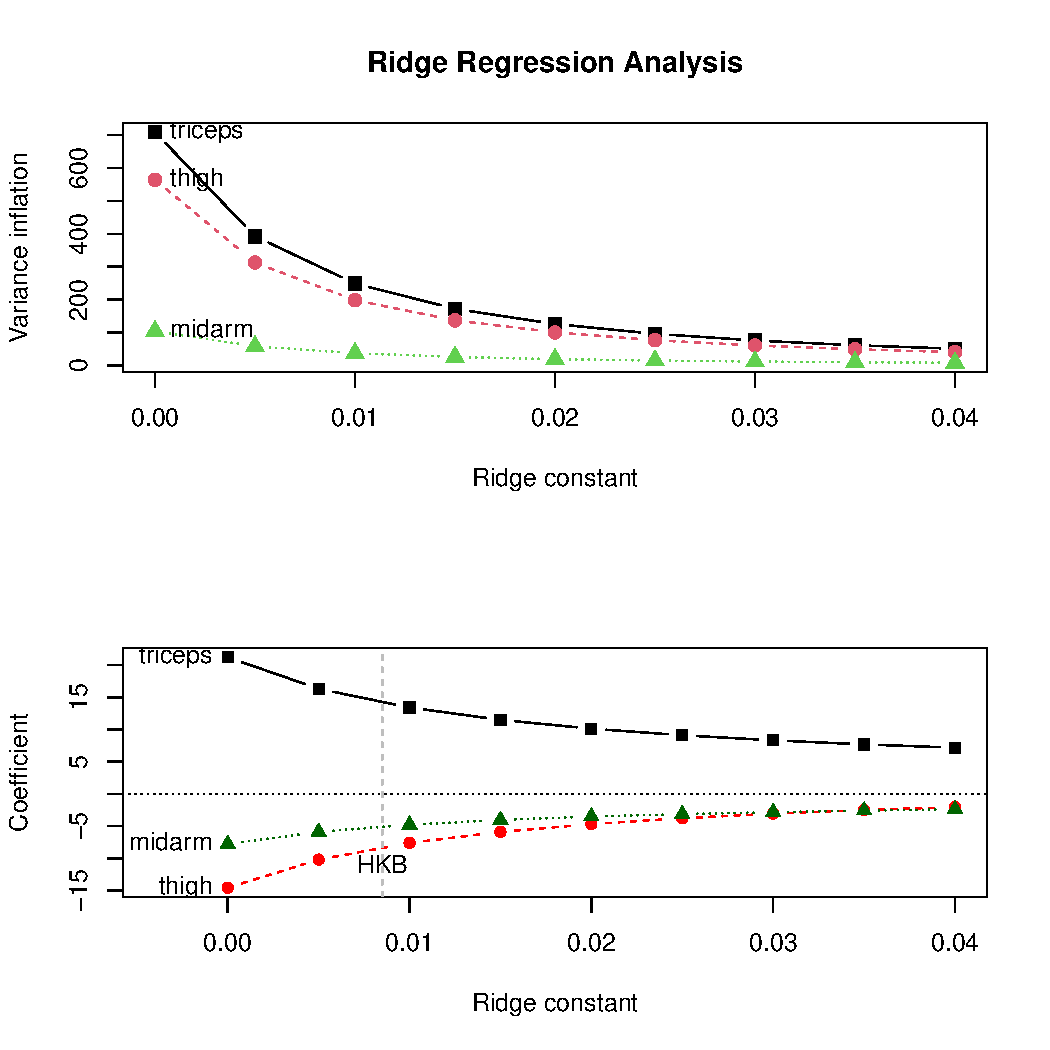
\includegraphics[width=0.6\textwidth]{figure/unnamed-chunk-2-1} 

}



\end{knitrout}

Our summary tells us that our OLS model would be:
\[\hat{Y} = 0.58003 X + 56.15693\]
where $X$ is our age.

\begin{knitrout}
\definecolor{shadecolor}{rgb}{0.969, 0.969, 0.969}\color{fgcolor}\begin{kframe}
\begin{alltt}
\hlstd{stat5100}\hlopt{::}\hlkwd{brown_forsythe_lm}\hlstd{(bp_lm)}
\end{alltt}
\begin{verbatim}
## [1] "Brown-forsythe test for constant variance in the residuals:"
## [1] "T-statistic: -2.7855, p-value: 0.0074"
\end{verbatim}
\begin{alltt}
\hlstd{stat5100}\hlopt{::}\hlkwd{cor_normality_lm}\hlstd{(bp_lm)}
\end{alltt}
\begin{verbatim}
## Correlation test of normality:
##                   resid expected_norm
## resid         1.0000000     0.9962478
## expected_norm 0.9962478     1.0000000
## 
## Total observations: 54
## Make sure to consult with table B.6 for your final result.
\end{verbatim}
\end{kframe}
\end{knitrout}

Very clearly, it looks like there is nonconstant variance in the residuals. To resolve this, we will use weighted least squares. What we do is we estimate the absolute value of the residual at each value of $X$ (age) with another regression model, and then using those estimates we can weight another model that predicts bp from age.

\begin{knitrout}
\definecolor{shadecolor}{rgb}{0.969, 0.969, 0.969}\color{fgcolor}\begin{kframe}
\begin{alltt}
\hlstd{absolute_residuals} \hlkwb{<-} \hlkwd{abs}\hlstd{(bp_lm}\hlopt{$}\hlstd{residuals)}
\hlstd{abs_resid_lm} \hlkwb{<-} \hlkwd{lm}\hlstd{(absolute_residuals} \hlopt{~} \hlstd{age,}
                   \hlkwc{data} \hlstd{=} \hlkwd{data.frame}\hlstd{(}\hlkwd{cbind}\hlstd{(absolute_residuals,}
                                           \hlkwc{age} \hlstd{= bpexample}\hlopt{$}\hlstd{age)))}
\hlstd{predicted_abs_resid} \hlkwb{<-} \hlstd{abs_resid_lm}\hlopt{$}\hlstd{fitted.values}

\hlcom{# Fit a new linear model with the weights obtained form predicted_abs_resid:}
\hlstd{weighted_bp_lm} \hlkwb{<-} \hlkwd{lm}\hlstd{(bp} \hlopt{~} \hlstd{age,} \hlkwc{data} \hlstd{= bpexample,}
                     \hlkwc{weights} \hlstd{=} \hlnum{1} \hlopt{/} \hlstd{predicted_abs_resid}\hlopt{^}\hlnum{2}\hlstd{)}
\hlkwd{summary}\hlstd{(weighted_bp_lm)}
\end{alltt}
\begin{verbatim}
## 
## Call:
## lm(formula = bp ~ age, data = bpexample, weights = 1/predicted_abs_resid^2)
## 
## Weighted Residuals:
##     Min      1Q  Median      3Q     Max 
## -2.0230 -0.9939 -0.0327  0.9250  2.2008 
## 
## Coefficients:
##             Estimate Std. Error t value Pr(>|t|)    
## (Intercept) 55.56577    2.52092  22.042  < 2e-16 ***
## age          0.59634    0.07924   7.526 7.19e-10 ***
## ---
## Signif. codes:  0 '***' 0.001 '**' 0.01 '*' 0.05 '.' 0.1 ' ' 1
## 
## Residual standard error: 1.213 on 52 degrees of freedom
## Multiple R-squared:  0.5214,	Adjusted R-squared:  0.5122 
## F-statistic: 56.64 on 1 and 52 DF,  p-value: 7.187e-10
\end{verbatim}
\end{kframe}
\end{knitrout}

Based upon the above result, our weighted least squares model would be:
\[\hat{Y} = 0.59634 X + 55.56577\]
where $X$ is the age. Notice below that if we look at the visual assumptions of our weighted model, it will look much the same as the original model. In this case, even though weighted least squares is ``better'' because our data violates the assumption of nonconstant variance in the residuals, the model ends up being incredibly similar to the OLS model, both in terms of visual assumption checks and in the $\beta$ coefficient estimates.

\begin{knitrout}
\definecolor{shadecolor}{rgb}{0.969, 0.969, 0.969}\color{fgcolor}\begin{kframe}
\begin{alltt}
\hlstd{stat5100}\hlopt{::}\hlkwd{visual_assumptions}\hlstd{(weighted_bp_lm)}
\end{alltt}
\end{kframe}

{\centering 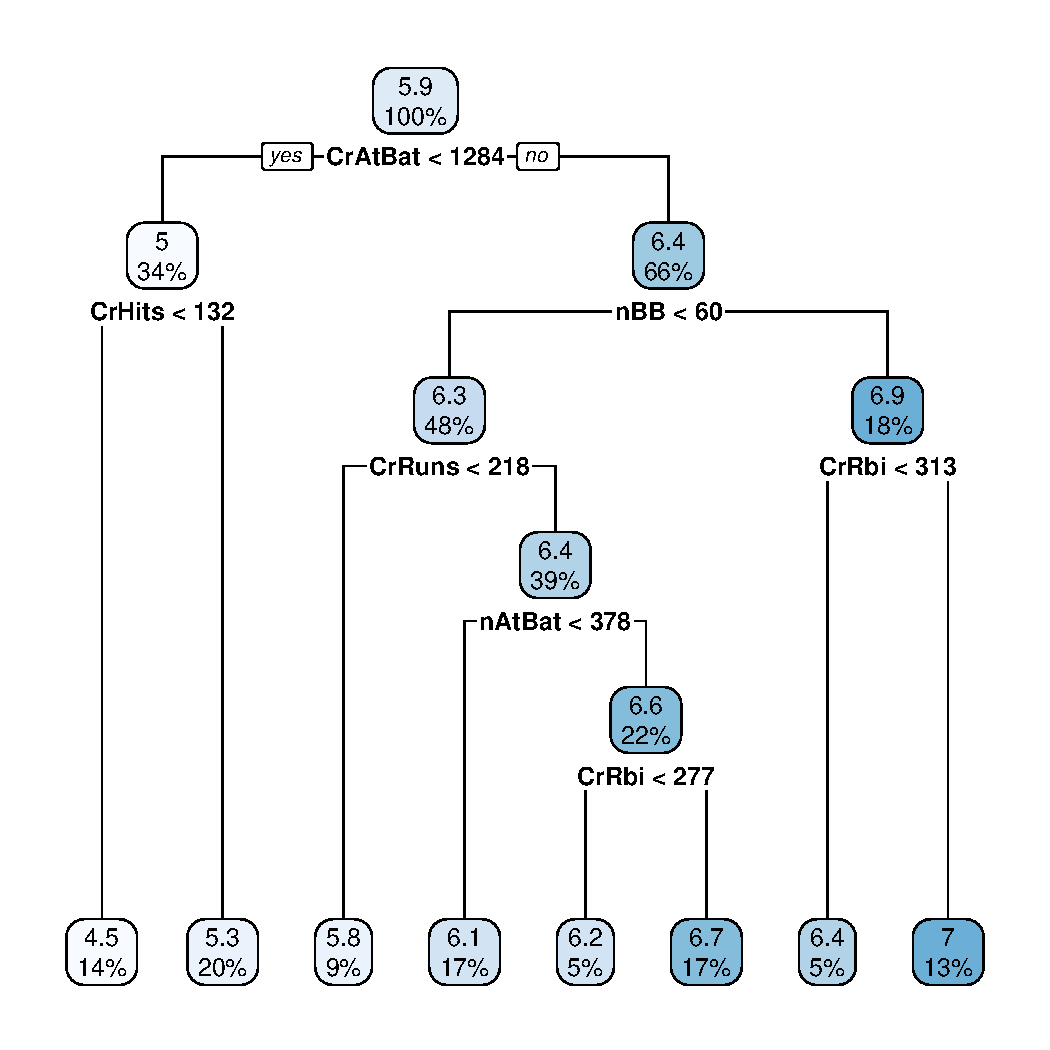
\includegraphics[width=0.6\textwidth]{figure/unnamed-chunk-5-1} 

}



\end{knitrout}

\newpage

\subsection*{Example 2: Iteratively reweighted least squares (IRLS) on Toluca dataset}
As part of a cost improvement program, the Toluca company wished to better understand the relationship between the lot size ($X$) and the total work hours ($Y$).

\begin{knitrout}
\definecolor{shadecolor}{rgb}{0.969, 0.969, 0.969}\color{fgcolor}\begin{kframe}
\begin{alltt}
\hlkwd{data}\hlstd{(toluca)}
\hlkwd{head}\hlstd{(toluca)}
\end{alltt}
\begin{verbatim}
##   lotsize workhours
## 1      80       399
## 2      30       121
## 3      50       221
## 4      90       376
## 5      70       361
## 6      60       224
\end{verbatim}
\end{kframe}
\end{knitrout}

Previously, OLS regression worked nicely on this dataset. However, to illustrate the usefulness of robust regression, we will intentionally contaminate the Toluca dataset with some outliers. We will eventually notice that fitting an OLS model on the contaminated data gives a very different model, but fitting a robust regression model on the contaminated data will give a very similar model to the OLS model fitted on the clean dataset.

\begin{knitrout}
\definecolor{shadecolor}{rgb}{0.969, 0.969, 0.969}\color{fgcolor}\begin{kframe}
\begin{alltt}
\hlcom{# Contaminate the data by tripling all the workhours if workhours is above 500}
\hlstd{toluca_c} \hlkwb{<-} \hlstd{toluca}
\hlstd{toluca_c}\hlopt{$}\hlstd{workhours[toluca_c}\hlopt{$}\hlstd{workhours} \hlopt{>} \hlnum{500}\hlstd{]} \hlkwb{<-}
  \hlnum{3}\hlopt{*}\hlstd{toluca_c}\hlopt{$}\hlstd{workhours[toluca_c}\hlopt{$}\hlstd{workhours} \hlopt{>} \hlnum{500}\hlstd{]}
\end{alltt}
\end{kframe}
\end{knitrout}

Let's look at scatterplots of the contaminated and uncontaminated data:

\begin{knitrout}
\definecolor{shadecolor}{rgb}{0.969, 0.969, 0.969}\color{fgcolor}\begin{kframe}
\begin{alltt}
\hlkwd{plot}\hlstd{(toluca}\hlopt{$}\hlstd{lotsize, toluca}\hlopt{$}\hlstd{workhours,} \hlkwc{xlab} \hlstd{=} \hlstr{"Lot size"}\hlstd{,} \hlkwc{ylab} \hlstd{=} \hlstr{"Work hours"}\hlstd{,}
     \hlkwc{main} \hlstd{=} \hlstr{"Uncontaminated Data"}\hlstd{)}
\hlkwd{plot}\hlstd{(toluca_c}\hlopt{$}\hlstd{lotsize, toluca_c}\hlopt{$}\hlstd{workhours,} \hlkwc{xlab} \hlstd{=} \hlstr{"Lot size"}\hlstd{,} \hlkwc{ylab} \hlstd{=} \hlstr{"Work hours"}\hlstd{,}
     \hlkwc{main} \hlstd{=} \hlstr{"Contaminated Data"}\hlstd{)}
\end{alltt}
\end{kframe}

{\centering 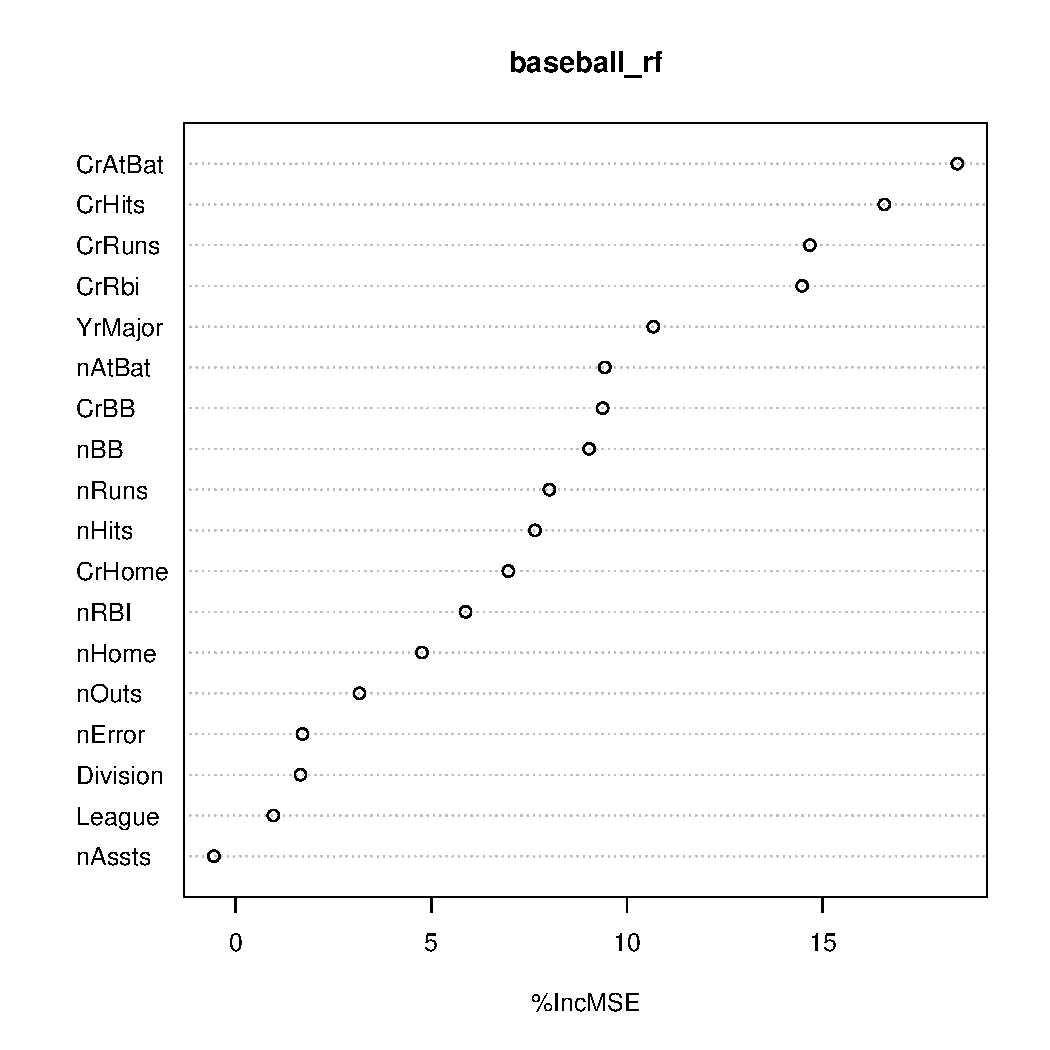
\includegraphics[width=0.45\textwidth]{figure/unnamed-chunk-8-1} 
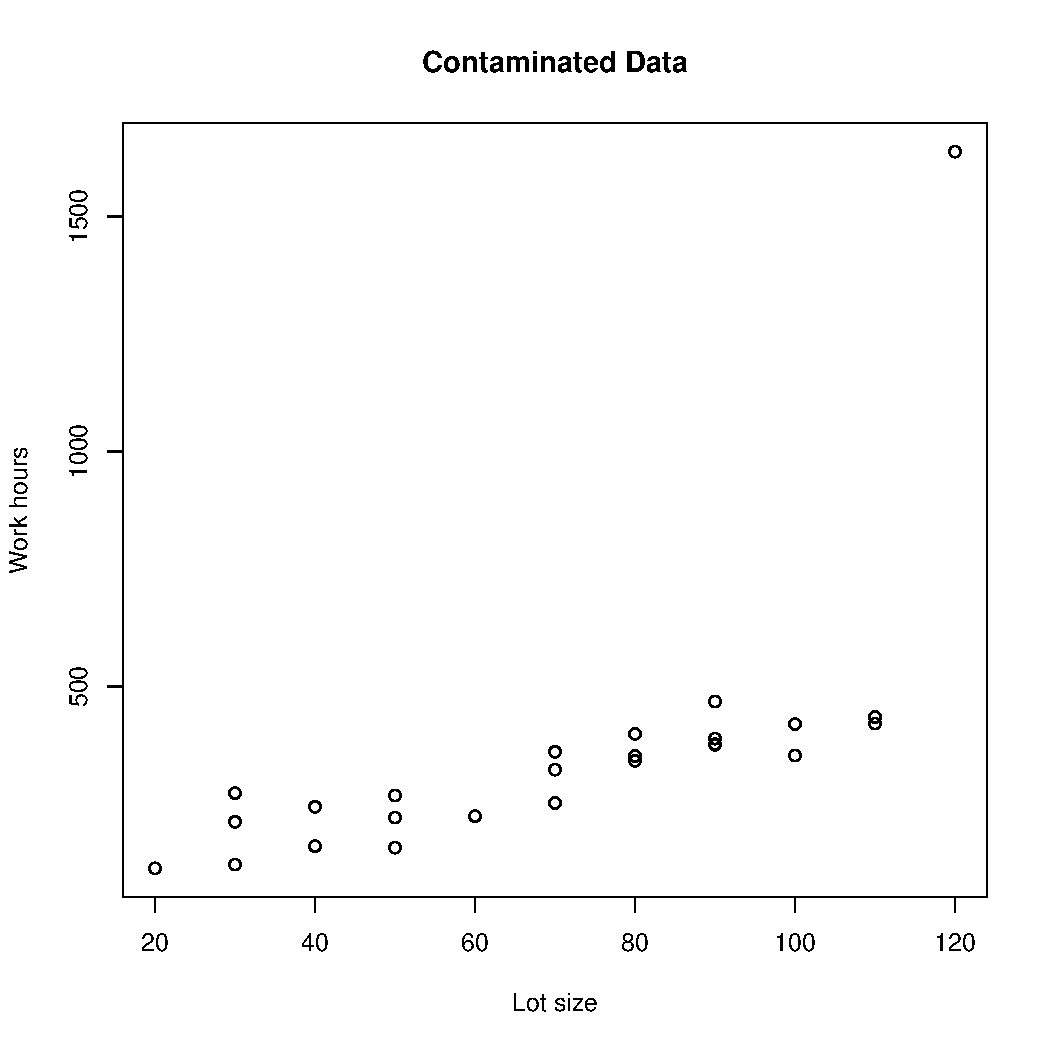
\includegraphics[width=0.45\textwidth]{figure/unnamed-chunk-8-2} 

}



\end{knitrout}

Now, we are going to use robust regression using Tukey's Bisquare weight. From our notes, the bisquare weighting function looks like
\[w(u) = \begin{cases}
\left( 1 - \left( \frac{u}{c} \right)^2 \right)^2 & \quad \text{if } |u| \le c \\
0 & \quad \text{otherwise}
\end{cases}\]
where $u$ is a standardized residual. Let's take a look at what the bisquare weight looks like for $c = 1.345$:

\begin{knitrout}
\definecolor{shadecolor}{rgb}{0.969, 0.969, 0.969}\color{fgcolor}\begin{kframe}
\begin{alltt}
\hlstd{c} \hlkwb{<-} \hlnum{1.345}
\hlstd{u} \hlkwb{<-} \hlkwd{seq}\hlstd{(}\hlopt{-}\hlnum{2}\hlstd{,} \hlnum{2}\hlstd{,} \hlkwc{by} \hlstd{=} \hlnum{0.01}\hlstd{)}
\hlstd{w} \hlkwb{<-} \hlstd{(}\hlnum{1} \hlopt{-} \hlstd{(u}\hlopt{/}\hlstd{c)}\hlopt{^}\hlnum{2}\hlstd{)}\hlopt{^}\hlnum{2}
\hlstd{w[}\hlkwd{abs}\hlstd{(u)} \hlopt{>=} \hlstd{c]} \hlkwb{<-} \hlnum{0}

\hlkwd{plot}\hlstd{(u, w,} \hlkwc{type} \hlstd{=} \hlstr{"l"}\hlstd{,} \hlkwc{main} \hlstd{=} \hlstr{"Bisquare weight function"}\hlstd{,}
     \hlkwc{xlab} \hlstd{=} \hlstr{"Standardized residual"}\hlstd{,} \hlkwc{ylab} \hlstd{=} \hlstr{"Bisquare weight"}\hlstd{)}
\end{alltt}
\end{kframe}

{\centering 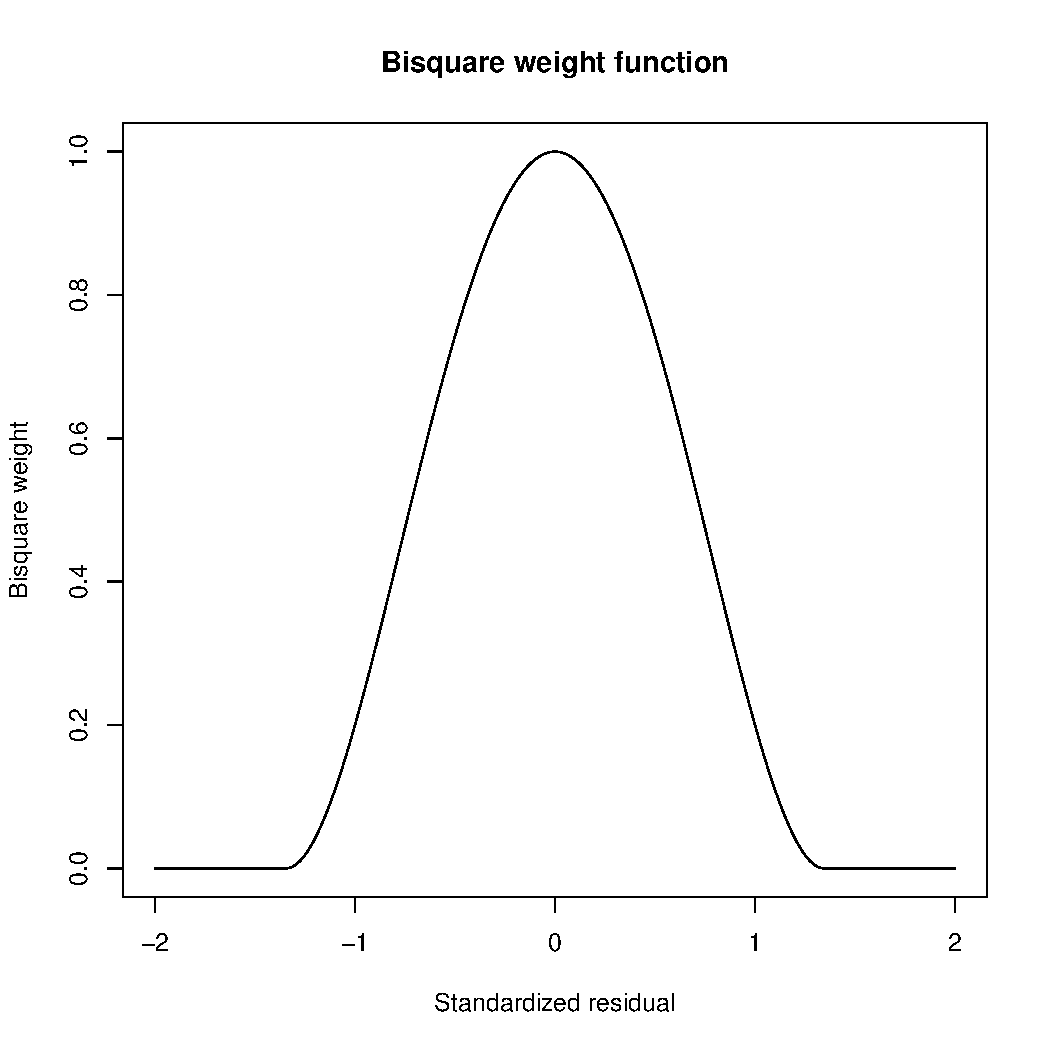
\includegraphics[width=0.6\textwidth]{figure/unnamed-chunk-9-1} 

}



\end{knitrout}

Now, let's fit the following models:
\begin{enumerate}
  \item OLS regression on original data
  \item OLS regression on contaminated data
  \item Robust regression with bisquare weight on contaminated data
\end{enumerate}

\begin{knitrout}
\definecolor{shadecolor}{rgb}{0.969, 0.969, 0.969}\color{fgcolor}\begin{kframe}
\begin{alltt}
\hlcom{# Model 1 (OLS on original data):}
\hlstd{toluca_ols} \hlkwb{<-} \hlkwd{lm}\hlstd{(workhours} \hlopt{~} \hlstd{lotsize,} \hlkwc{data} \hlstd{= toluca)}
\hlkwd{summary}\hlstd{(toluca_ols)}
\end{alltt}
\begin{verbatim}
## 
## Call:
## lm(formula = workhours ~ lotsize, data = toluca)
## 
## Residuals:
##     Min      1Q  Median      3Q     Max 
## -83.876 -34.088  -5.982  38.826 103.528 
## 
## Coefficients:
##             Estimate Std. Error t value Pr(>|t|)    
## (Intercept)   62.366     26.177   2.382   0.0259 *  
## lotsize        3.570      0.347  10.290 4.45e-10 ***
## ---
## Signif. codes:  0 '***' 0.001 '**' 0.01 '*' 0.05 '.' 0.1 ' ' 1
## 
## Residual standard error: 48.82 on 23 degrees of freedom
## Multiple R-squared:  0.8215,	Adjusted R-squared:  0.8138 
## F-statistic: 105.9 on 1 and 23 DF,  p-value: 4.449e-10
\end{verbatim}
\begin{alltt}
\hlcom{# Model 2 (OLS on contaminated data):}
\hlstd{toluca_c_ols} \hlkwb{<-} \hlkwd{lm}\hlstd{(workhours} \hlopt{~} \hlstd{lotsize,} \hlkwc{data} \hlstd{= toluca_c)}
\hlkwd{summary}\hlstd{(toluca_c_ols)}
\end{alltt}
\begin{verbatim}
## 
## Call:
## lm(formula = workhours ~ lotsize, data = toluca_c)
## 
## Residuals:
##     Min      1Q  Median      3Q     Max 
## -192.79 -103.96  -32.96   18.15  965.65 
## 
## Coefficients:
##             Estimate Std. Error t value Pr(>|t|)    
## (Intercept)  -86.984    120.908  -0.719 0.479126    
## lotsize        6.328      1.603   3.948 0.000639 ***
## ---
## Signif. codes:  0 '***' 0.001 '**' 0.01 '*' 0.05 '.' 0.1 ' ' 1
## 
## Residual standard error: 225.5 on 23 degrees of freedom
## Multiple R-squared:  0.404,	Adjusted R-squared:  0.3781 
## F-statistic: 15.59 on 1 and 23 DF,  p-value: 0.0006393
\end{verbatim}
\begin{alltt}
\hlcom{# Model 3 (Robust regression on contaminated data)}
\hlstd{toluca_c_robust} \hlkwb{<-} \hlstd{MASS}\hlopt{::}\hlkwd{rlm}\hlstd{(workhours} \hlopt{~} \hlstd{lotsize,} \hlkwc{data} \hlstd{= toluca_c,}
                             \hlkwc{method} \hlstd{=} \hlkwd{c}\hlstd{(}\hlstr{"MM"}\hlstd{))}
\hlkwd{summary}\hlstd{(toluca_c_robust)}
\end{alltt}
\begin{verbatim}
## 
## Call: rlm(formula = workhours ~ lotsize, data = toluca_c, method = c("MM"))
## Residuals:
##        Min         1Q     Median         3Q        Max 
##  -83.19265  -24.53354   -0.07146   38.02706 1158.26944 
## 
## Coefficients:
##             Value   Std. Error t value
## (Intercept) 69.0941 27.4773     2.5146
## lotsize      3.4220  0.3642     9.3958
## 
## Residual standard error: 54.72 on 23 degrees of freedom
\end{verbatim}
\end{kframe}
\end{knitrout}

Let us now plot all three regression lines on the contaminated dataset.

\begin{knitrout}
\definecolor{shadecolor}{rgb}{0.969, 0.969, 0.969}\color{fgcolor}\begin{kframe}
\begin{alltt}
\hlcom{# First, get coefficient estimates from the models.}
\hlstd{orig_coef} \hlkwb{<-} \hlstd{toluca_ols}\hlopt{$}\hlstd{coefficients}
\hlstd{contam_coef} \hlkwb{<-} \hlstd{toluca_c_ols}\hlopt{$}\hlstd{coefficients}
\hlstd{robust_coef} \hlkwb{<-} \hlstd{toluca_c_robust}\hlopt{$}\hlstd{coefficients}

\hlkwd{plot}\hlstd{(toluca_c}\hlopt{$}\hlstd{lotsize, toluca_c}\hlopt{$}\hlstd{workhours,} \hlkwc{main} \hlstd{=} \hlstr{"Comparison of methods"}\hlstd{,}
     \hlkwc{xlab} \hlstd{=} \hlstr{"Lot size"}\hlstd{,} \hlkwc{ylab} \hlstd{=} \hlstr{"Work hours"}\hlstd{)}
\hlkwd{abline}\hlstd{(}\hlkwc{a} \hlstd{= orig_coef[}\hlnum{1}\hlstd{],} \hlkwc{b} \hlstd{= orig_coef[}\hlnum{2}\hlstd{],} \hlkwc{col} \hlstd{=} \hlstr{"blue"}\hlstd{)}
\hlkwd{abline}\hlstd{(}\hlkwc{a} \hlstd{= contam_coef[}\hlnum{1}\hlstd{],} \hlkwc{b} \hlstd{= contam_coef[}\hlnum{2}\hlstd{],} \hlkwc{col} \hlstd{=} \hlstr{"red"}\hlstd{)}
\hlkwd{abline}\hlstd{(}\hlkwc{a} \hlstd{= robust_coef[}\hlnum{1}\hlstd{],} \hlkwc{b} \hlstd{= robust_coef[}\hlnum{2}\hlstd{],} \hlkwc{col} \hlstd{=} \hlstr{"violet"}\hlstd{)}
\hlkwd{legend}\hlstd{(}\hlstr{"topleft"}\hlstd{,} \hlkwc{legend} \hlstd{=} \hlkwd{c}\hlstd{(}\hlstr{"Uncontaminated OLS"}\hlstd{,} \hlstr{"Contaminated OLS"}\hlstd{,} \hlstr{"Contaminated Robust"}\hlstd{)}
       \hlstd{,} \hlkwc{col} \hlstd{=} \hlkwd{c}\hlstd{(}\hlstr{"blue"}\hlstd{,} \hlstr{"red"}\hlstd{,} \hlstr{"violet"}\hlstd{),} \hlkwc{pch} \hlstd{=} \hlnum{16}\hlstd{)}
\end{alltt}
\end{kframe}

{\centering 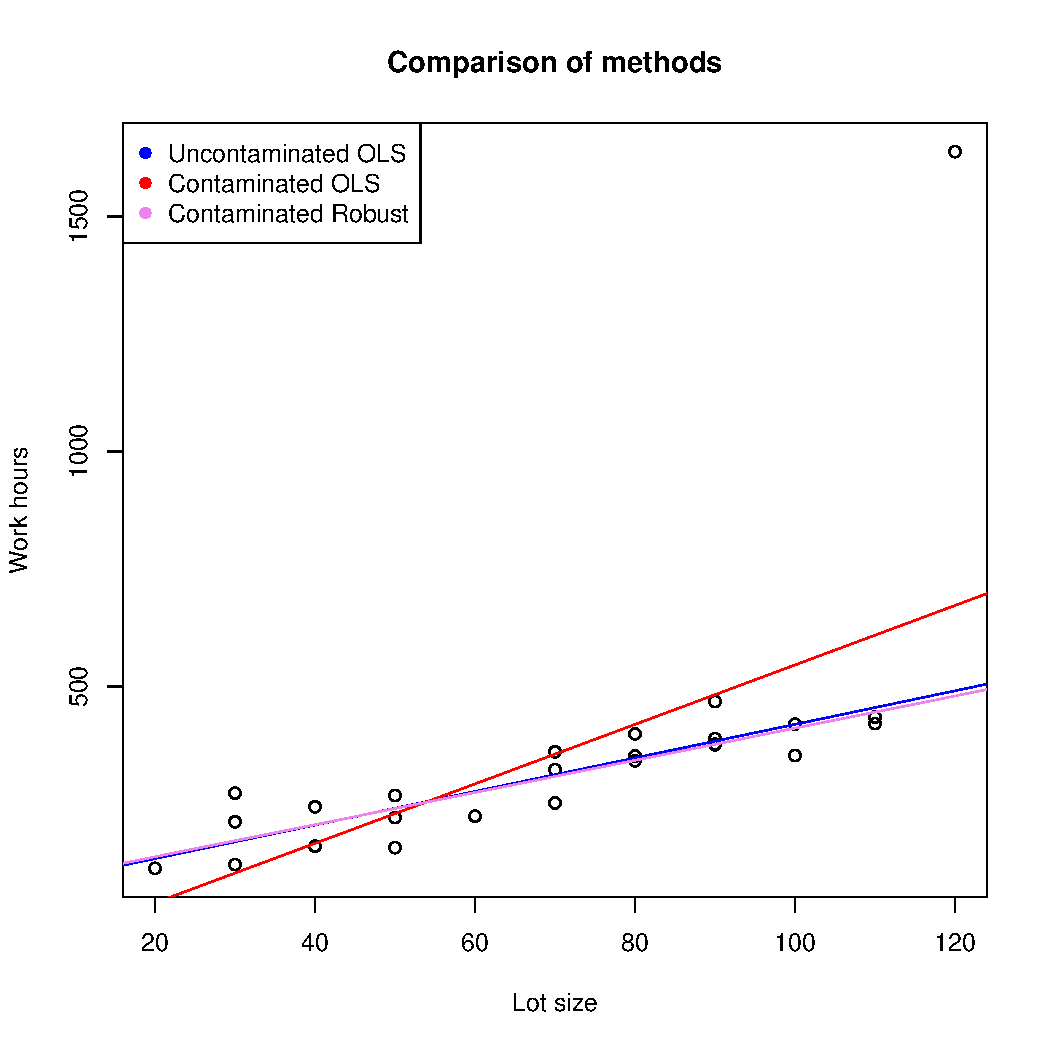
\includegraphics[width=0.6\textwidth]{figure/unnamed-chunk-11-1} 

}



\end{knitrout}

In the above plot, note that the contaminated robust line is essentially the same as the uncontaminated OLS line. The contaminated OLS line is clearly different, primarily because it is getting pulled upward so much by the outlier point in the contaminated dataset.

\newpage

\subsection*{Example 3.1: Nonlinear regression}

Here, we will assume a model form of the following:
\[Y = \beta_0 + \beta_1 X_1^{\beta_2} - \beta_3 e^{\beta_4 X_2} + \epsilon\]

We will try our nonlinear regression model on some randomly generated data:
\begin{knitrout}
\definecolor{shadecolor}{rgb}{0.969, 0.969, 0.969}\color{fgcolor}\begin{kframe}
\begin{alltt}
\hlcom{# Set a random seed}
\hlkwd{set.seed}\hlstd{(}\hlnum{141414}\hlstd{)}

\hlstd{x1} \hlkwb{<-} \hlnum{10} \hlopt{+} \hlnum{10}\hlopt{*}\hlkwd{runif}\hlstd{(}\hlkwc{n} \hlstd{=} \hlnum{50}\hlstd{)}
\hlstd{x2} \hlkwb{<-} \hlnum{1} \hlopt{+} \hlnum{2}\hlopt{*}\hlkwd{runif}\hlstd{(}\hlkwc{n} \hlstd{=} \hlnum{50}\hlstd{)}
\hlstd{error} \hlkwb{<-} \hlnum{10}\hlopt{*}\hlkwd{rnorm}\hlstd{(}\hlkwc{n} \hlstd{=} \hlnum{50}\hlstd{)}

\hlcom{# Define a true relationship with Y: (beta0 = 50, beta1 = 10, beta2 = 2,}
\hlcom{# beta3 = 16, beta4 = 2)}
\hlstd{y} \hlkwb{<-} \hlnum{50} \hlopt{+} \hlnum{10}\hlopt{*}\hlstd{x1}\hlopt{^}\hlnum{2} \hlopt{-} \hlnum{16}\hlopt{*}\hlkwd{exp}\hlstd{(}\hlnum{2}\hlopt{*}\hlstd{x2)} \hlopt{+} \hlstd{error}

\hlcom{# Now look at scatterplots of X1 and Y and X2 and Y:}
\hlkwd{plot}\hlstd{(x1, y)}
\hlkwd{plot}\hlstd{(x2, y)}
\end{alltt}
\end{kframe}

{\centering 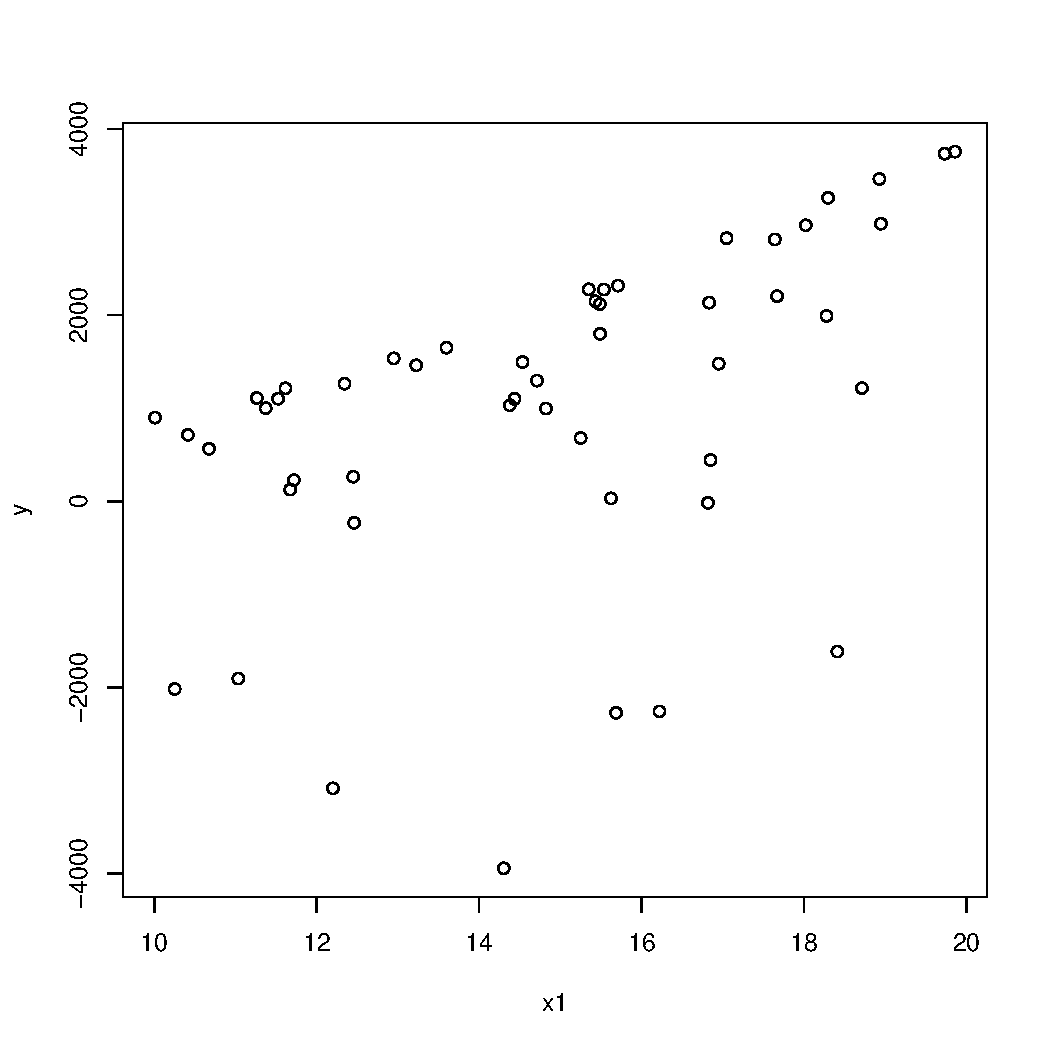
\includegraphics[width=0.45\textwidth]{figure/unnamed-chunk-12-1} 
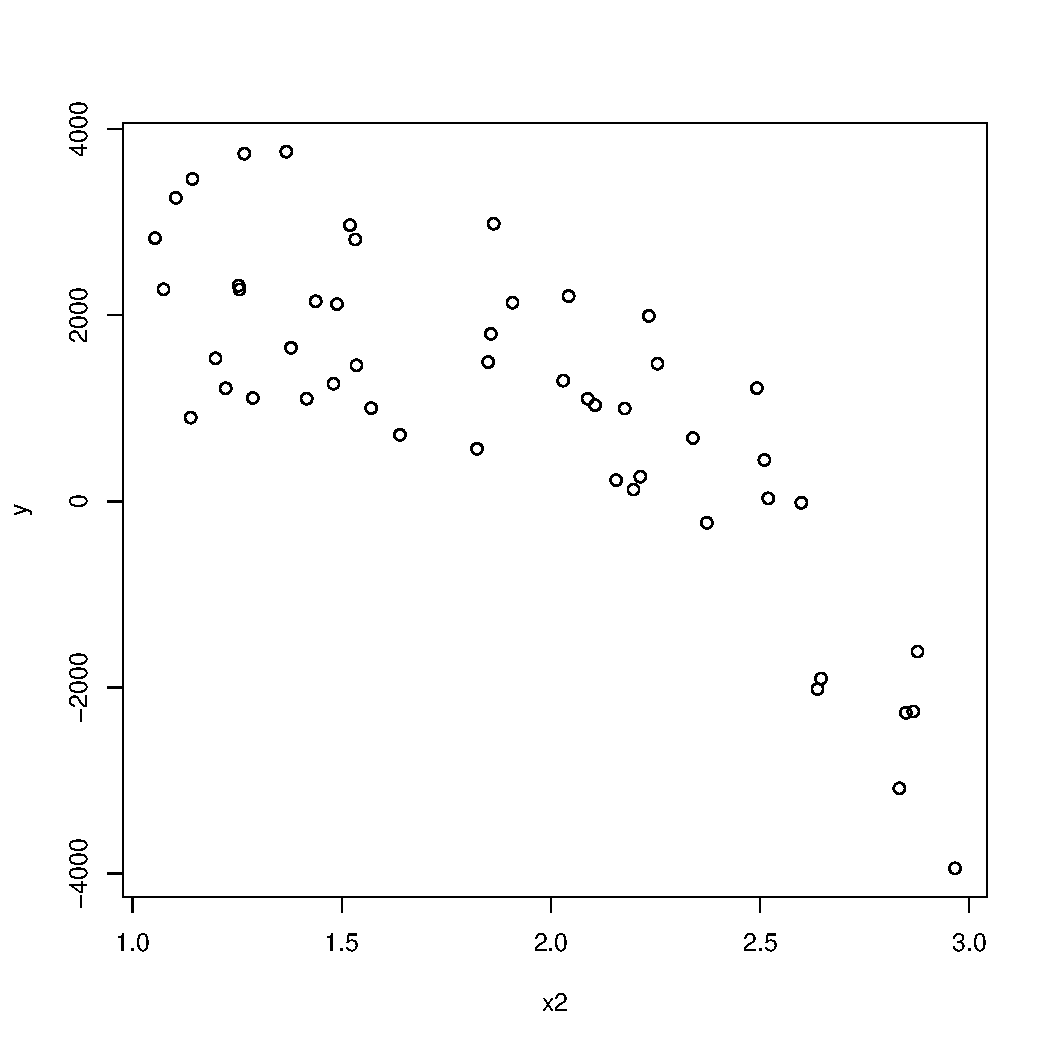
\includegraphics[width=0.45\textwidth]{figure/unnamed-chunk-12-2} 

}



\end{knitrout}

\begin{knitrout}
\definecolor{shadecolor}{rgb}{0.969, 0.969, 0.969}\color{fgcolor}\begin{kframe}
\begin{alltt}
\hlcom{# Train our nonlinear regression model}
\hlstd{simulated_nls} \hlkwb{<-} \hlkwd{nls}\hlstd{(y} \hlopt{~} \hlstd{b0} \hlopt{+} \hlstd{b1}\hlopt{*}\hlstd{x1}\hlopt{^}\hlstd{b2} \hlopt{-} \hlstd{b3}\hlopt{*}\hlkwd{exp}\hlstd{(b4}\hlopt{*}\hlstd{x2),}
                     \hlkwc{start} \hlstd{=} \hlkwd{list}\hlstd{(}\hlkwc{b0} \hlstd{=} \hlnum{100}\hlstd{,} \hlkwc{b1} \hlstd{=} \hlnum{8}\hlstd{,} \hlkwc{b2} \hlstd{=} \hlnum{3}\hlstd{,} \hlkwc{b3} \hlstd{=} \hlopt{-}\hlnum{20}\hlstd{,} \hlkwc{b4} \hlstd{=} \hlnum{4}\hlstd{))}
\hlkwd{summary}\hlstd{(simulated_nls)}
\end{alltt}
\begin{verbatim}
## 
## Formula: y ~ b0 + b1 * x1^b2 - b3 * exp(b4 * x2)
## 
## Parameters:
##     Estimate Std. Error t value Pr(>|t|)    
## b0 68.362945  22.559272    3.03  0.00404 ** 
## b1  9.506840   0.652230   14.58  < 2e-16 ***
## b2  2.014894   0.021366   94.30  < 2e-16 ***
## b3 15.773176   0.234294   67.32  < 2e-16 ***
## b4  2.004962   0.005068  395.60  < 2e-16 ***
## ---
## Signif. codes:  0 '***' 0.001 '**' 0.01 '*' 0.05 '.' 0.1 ' ' 1
## 
## Residual standard error: 10.66 on 45 degrees of freedom
## 
## Number of iterations to convergence: 17 
## Achieved convergence tolerance: 8.145e-08
\end{verbatim}
\end{kframe}
\end{knitrout}

Based upon the above summary, our final function guess would be the following:
\[\hat{Y} = 68.363 + 9.507 X_1^{2.015} - 15.773 e^{2.005 X_2}\]
Compare this with the true equation form:
\[Y = 50 + 10 X_1^2 - 16 e^{2 X_2} + \epsilon\]

\end{document}
